\chapter{Đại số Boolean}

Boolean (hay luận lý) chỉ giá trị đúng hoặc sai của mệnh đề nào đó. 
Theo cách hiểu cơ bản, boolean gồm 2 giá trị 0 hoặc 1 (sai hoặc đúng).

\section{Hàm Boolean}

Hàm boolean $f$ đối với các biến $x_1, x_2, \ldots, x_n$ là hàm số 
nhận giá trị trong $\{0, 1\}^n$ và trả về giá trị thuộc $\{0, 1\}$.

Nghĩa là $f: \{0,1\}^n \mapsto \{0, 1\}$

\section{Các loại hàm boolean}

\begin{definition}[Đa thức Zhegalkin]
    Với hàm boolean $n$ biến $f(x_1, x_2, \ldots, x_n)$, đa thức Zhegalkin tương ứng với hàm bool đó là cách biểu diễn
    đa thức đó dưới dạng tổng các tích như sau
    \begin{equation}
        f(x_1, x_2, \ldots, x_n) = a_0 \oplus a_1 x_1 
        \oplus a_2 x_2 \oplus a_3 x_1 x_2 \oplus \ldots 
        \oplus a_k x_1 x_2 \ldots x_n
    \end{equation}
    với $a_i \in \{0, 1\}$. Ta thấy rằng có $n$ biến, do đó có 
    $2^n$ hệ số $a_i$ ($k = 2^n$).
\end{definition}

\begin{example}
    Cho hàm bool $f(x, y) = x \vee y$. Ta có bảng chân trị sau
    \begin{table}[ht]
        \centering
        \begin{tabular}{c c c}
            $x$ & $y$ & $f(x, y)$ \\
            0 & 0 & 0 \\
            0 & 1 & 1 \\
            1 & 0 & 1 \\
            1 & 1 & 1 \\
        \end{tabular}
    \end{table}

    Bảng chân trị này tương đương với đa thức Zhegalkin
    \[f(x, y) = x \oplus y \oplus xy\]
\end{example}

Để tìm đa thức Zhegalkin của một hàm boolean từ bảng chân trị, ta 
có thể dùng phương pháp tam giác. Ở hàng đầu ta viết các phần
tử bảng chân trị từ trái sang phải. Với $n$ biến sẽ có $2^n$ ô.
Hàng thứ hai có $2^n-1$ ô. Phần tử dưới sẽ bằng XOR của 2 phần tử 
ngay trên nó (tạo thành tam giác). Tiếp tục như vậy tới khi
ta có hàng cuối chỉ có 1 ô.

\begin{figure}[ht]
    \centering
    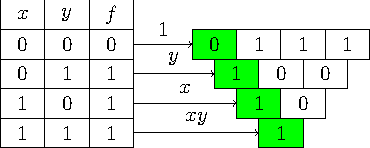
\includegraphics{pics/boolean/zhegalkin1.pdf}
    \caption{Phương pháp tam giác}
\end{figure}

Khi đó, tương ứng với các biến, nếu biến đó là 1 thì hạng tử chứa
biến đó, 0 thì không ghi. Ở ví dụ trên, nếu $(x, y) = (0, 0)$ 
thì không có gì (phần tử 1), $(x, y) = (0, 1)$ tương ứng với hạng tử $y$
trong đa thức Zhegalkin, $(x, y) = (1, 0)$ tương ứng hạng
tử $x$. Cuối cùng $(x, y) = (1, 1)$ tương ứng hạng tử $xy$.

Hệ số trước mỗi hạng tử là phần tử đầu tiên bên trái theo bảng
kim tự tháp. Như vậy đa thức Zhegalkin là:
\begin{equation}
    f(x, y) = 0 \cdot 1 \oplus 1 \cdot y \oplus 1 \cdot x \oplus 
        1 \cdot xy = x \oplus y \oplus xy
\end{equation}

Đa thức Zhegalkin đóng vai trò quan trọng trong nhiều lĩnh vực,
bao gồm cả toán học, vật lý, khoa học máy tính, vì AND và XOR
là hai toán tử đại số cơ bản.